%% ============================================================
%% 分片 26：原文第 10 节「The Bogomolny Equations And The Space Of Hecke Modifications」（原文 glshort.tex 起于第 8120 行）
%% 由 tools/harvmac2tex.py 从 arXiv 源码（hep-th/0604151v3）自动生成。
%% 只译英文散文；公式、编号、\label、\cite 一律不改。
%% ============================================================

\section{ The Bogomolny Equations And The Space Of Hecke
Modifications}

\label{sec:bogeqheck}

In this section, we return to the Bogomolny equations with
singularities and study them more closely. The first goal is to
exhibit the space of Hecke modifications of a given type as a
moduli space of solutions of the Bogomolny equations, with
suitable boundary conditions. This will enable us to get a clear
picture of many relatively subtle aspects of the spaces of Hecke
modifications. Then we relax the assumption of time-reversal
invariance and consider the complexified or extended Bogomolny
equations. These extended equations enable one to define the Hecke
transform of an arbitrary $A$-brane on $\MH(G,C)$ and therefore
are the important ones for geometric Langlands duality.

\subsection{Boundary Conditions}

\label{sec:boundcon}

We will study the Bogomolny equations on  a $G$-bundle $E$ over a
three-manifold $W=I\times C$ (as usual, $I$ is an interval and $C$
a Riemann surface, and there are prescribed singularities at
points $p_i\in W$ where 't Hooft operators are inserted).  We
write $C_-$ and $C_+$ for the two ends of $W$,  $E_-$ and $E_+$
for the restriction of $E$ to the two ends, and $A_-$ and $A_+$
for the restrictions of the connection $A$.

\begin{figure}[htbp]
\centering
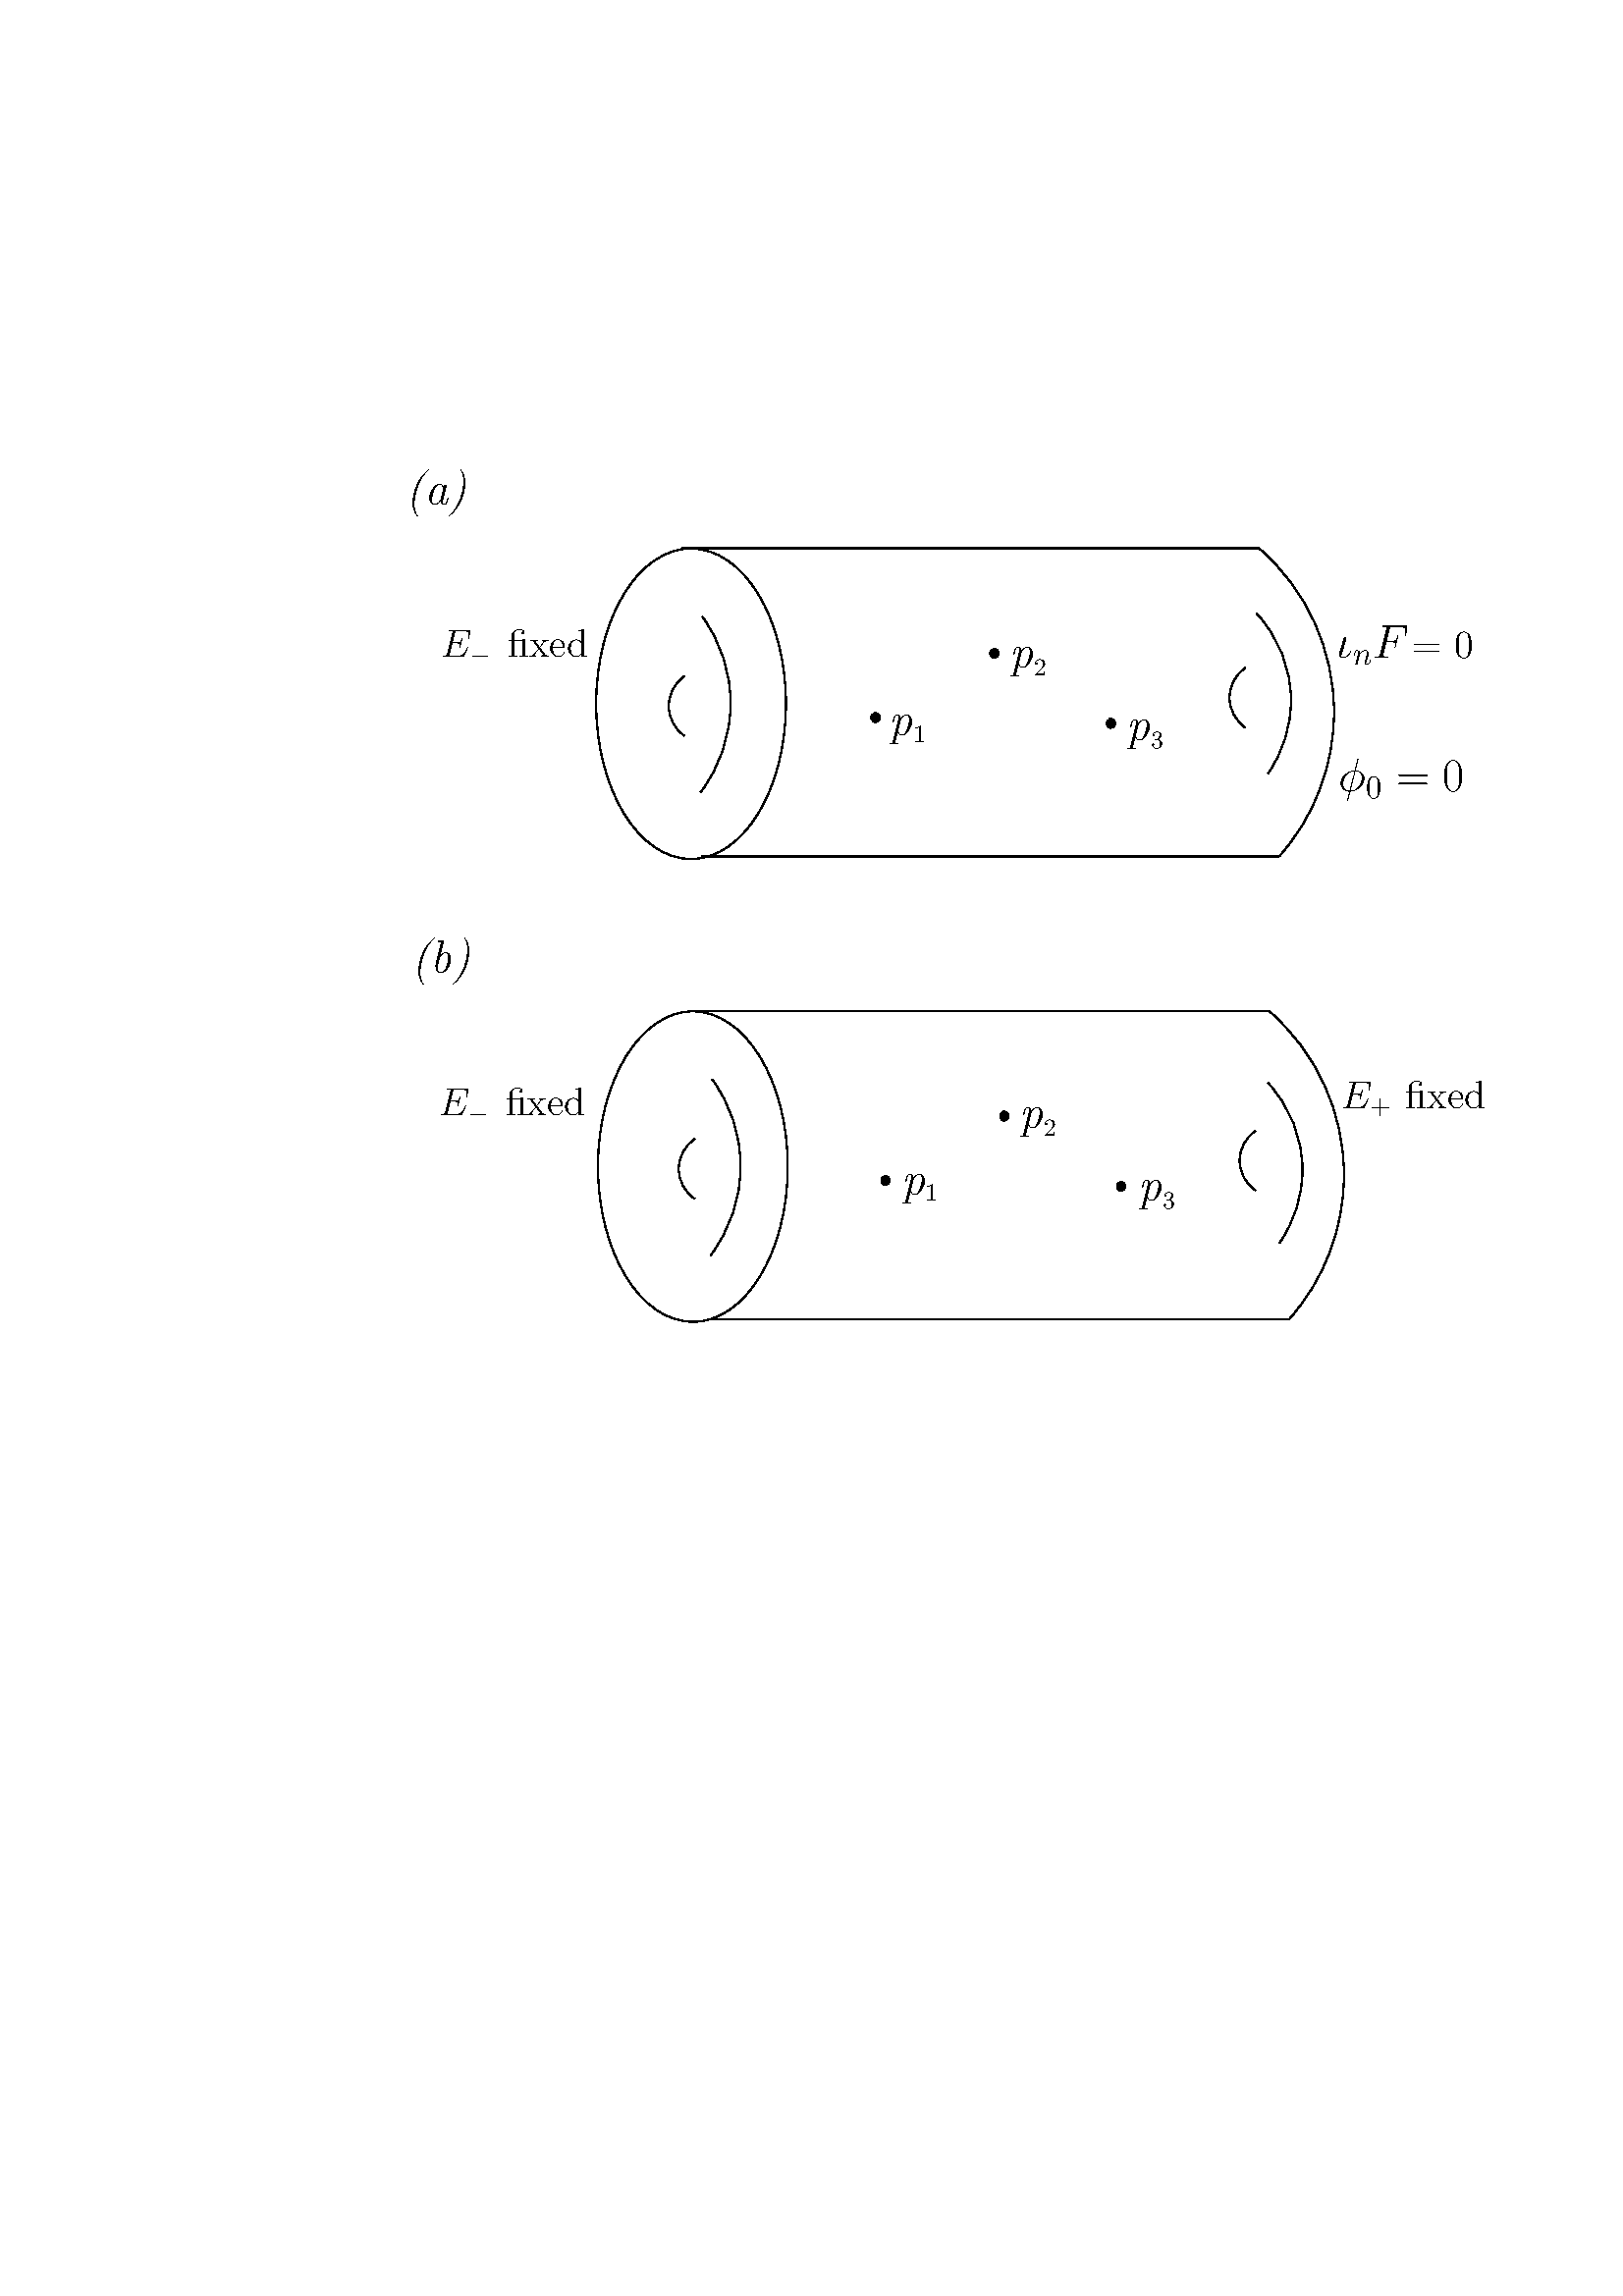
\includegraphics[width=0.75\linewidth]{figures/gla7-4.png}
\caption{(a) On the three-manifold $W=I\times C$ with 't Hooft operator insertions, a bundle $E_-$ is specified on the left, and one wishes to determine possible Hecke modifications $E_+$ that may appear on the right. On the left, the connection $A_-$ obeys Dirichlet boundary conditions and $\phi_0$ is undetermined; on the right, their roles are reversed. (b) To describe a fiber of the Hecke correspondence, one specifies both $E_-$ and $E_+$ and leaves $\phi_0$ undetermined at each end.（原文 Fig.~15）}
\label{fig:utampo}
\end{figure}

There are two closely related problems that we might consider. One
natural question  is to describe the action of the 't Hooft/Hecke
operators on bundles, and the second is to describe the Hecke
correspondence.

For the first problem (\utampo(a)), we specify a bundle $E_-$ at
the left end of $W$ and then ask what bundle $E_+$ can appear at
the other end as a result of solving the Bogomolny equations with
singularities. In this way we should recover the space of Hecke
modifications, as described in section 第~\ref{sec:theck}~节.  An alternative
problem (\utampo(b)) is to try to describe the Hecke
correspondence, which parametrizes pairs of bundles with a
suitable Hecke relation. We will describe boundary conditions
appropriate for either of these two problems.

To specify the bundle $E_-$, we specify the gauge field $A_-$ on
$C_-$. We want to specify an actual bundle $E_-$, not an
isomorphism class of bundles, so we specify an actual connection
$A_-$ on $C_-$. So we will only divide by gauge transformations
that are trivial on $C_-$.  It is convenient for some purposes to
assume that the bundle $E_-$ is stable, in which case we can
assume that the connection $A_-$ is flat.  We will not assume that
the output bundle $E_+$ that results from solving the Bogomolny
equations is stable.

We want the boundary conditions on $C_-$ to be elliptic (modulo
the gauge transformations). The simplest elliptic boundary
conditions in the Bogomolny equations are obtained by either
imposing Dirichlet boundary conditions on $A$ -- that is,
specifying its boundary values -- and leaving the boundary values
of $\phi_0$ unspecified, or vice-versa. If the boundary values of
$A$ are specified, then the Bogomolny equations determine the
normal derivative of $\phi_0$ at the boundary, and vice-versa. At
$E_-$, since we want to specify $A$, we leave $\phi_0$
unspecified.  If $A_-$ is flat, then the Bogomolny equations
require the normal derivative of $\phi_0$ to vanish at $C_-$.

At $C_+$, on the other hand, we want to allow all possible Hecke
modifications $E_+$ that may arise from $E_-$ by solving the
Bogomolny equations.  So the connection $A$ is unspecified on
$C_+$, and instead we set $\phi_0=0$ on $C_+$.   The Bogomolny
equations then require that $A$ obeys covariant Neumann boundary
conditions at $E_+$; that is, its  curvature $F(A)$ vanishes when
contracted with the normal vector to the boundary. We are only
interested in the output bundle $E_+$ up to gauge transformations,
so we allow the gauge transformations to be non-trivial on $C_+$.
These boundary conditions are summarized in \utampo(a). In section
第~\ref{sec:kahstr}~节, we will understand more deeply the naturalness of these
boundary conditions.

\par\medskip{\it The Hecke Correspondence}

What we have just described is the boundary condition that we will
generally use in employing the Bogomolny equations to study Hecke
operators. But we pause to discuss the differential geometric
analog of another formulation that is standard in algebraic
geometry. (The details are not needed for the rest of the paper.)
Instead of thinking of $E_-$ as input and $E_+$ as output, as we
have done above,  one can treat the two symmetrically by
describing the ``Hecke correspondence.'' In the usual formulation
in algebraic geometry, we let ${\rm Bun}_G$ be the ``stack'' of
all $G$-bundles over $C$, not necessarily stable. The Hecke
correspondence of type $^L\negthinspace w,z$ (for a weight
$^L\negthinspace w$ and a point $z\in C$) is then a variety ${\cal
Q}(^L\negthinspace w,z)$ that maps to ${\rm Bun}_G\times {\rm
Bun}_G$. The fiber of ${\cal Q}(^L\negthinspace w,z)$ over
$E_-\times E_+\in {\rm Bun}_G\times {\rm Bun}_G$ parametrizes ways
of obtaining $E_+$ from $E_-$ by a Hecke transformation of type
$^L\negthinspace w$ at $z$.

\def\EUPT{\eusm{PT}}
The relationship between $E_-$ and $E_+$ can be stated more
symmetrically, as $C_-$ and $C_+$ are exchanged by an
orientation-preserving automorphism $\EUPT$ that acts trivially on
$C$, exchanges the two ends of $I$, and also reverses the time
coordinate.   Such an automorphism maps $\phi$ to $\EUPT^*(\phi)$,
and maps an 't Hooft operator of weight $^L\negthinspace w$ to one
of weight $^L\negthinspace w'$, where $^L\negthinspace w'$ is a
dominant weight that is Weyl conjugate to $-{}^L\negthinspace w$.
So $E_+$ is produced from $E_-$ by a Hecke transformation of type
$^L\negthinspace w$ at $z$, or equivalently $E_-$ is produced from
$E_+$ by a Hecke transformation of type $^L\negthinspace w'$ at
$z$.

The fiber of the map ${\cal Q}({}^L\negthinspace w,z)$ to ${\rm
Bun}_G\times {\rm Bun}_G$ is generically empty if the weight
$^L\negthinspace w$ is small and the genus of $C$ is large. On the
other hand, for any $C$, this map is generically a fibration if
$^L\negthinspace w$ is large enough. One can extend the definition
of ${\cal Q}$ to allow several Hecke operators with specified
positions and weights, in which case the nature of the map ${\cal
Q}\to {\rm Bun}_G\times {\rm Bun}_G$ depends on the number and
weights of the 't Hooft operators.

In differential geometry, ${\rm Bun}_G$ corresponds to the space
$\EUA$ of all connections.  $\EUA$ is of course
infinite-dimensional, and ${\rm Bun}_G$ is an algebro-geometric
analog of an infinite-dimensional manifold (it includes bundles
that are arbitrarily unstable with no bound on the dimensions of
spaces of deformations and automorphism groups).  The Hecke
correspondence ${\cal Q}$ likewise is infinite-dimensional and
will not come from elliptic boundary conditions.  A
differential-geometric version of the Hecke correspondence is to
simply define ${\cal Q}$ as the space of all solutions of the
Bogomolny equations on $W=I\times C$, with specified
singularities, modulo gauge transformations that are trivial at
each end. The map of ${\cal Q}$ to $\EUA\times \EUA$ is obtained
by restricting a solution to the two ends of $W$.

${\cal Q}$ is infinite-dimensional, as in defining it we have
specified neither $A$ nor $\phi_0$ at either end; these boundary
conditions are not elliptic.  In differential geometry, it seems
more natural to define the fiber of the Hecke correspondence over
a pair of connections $A_-\times A_+\subset \EUA\times \EUA$. This
is the gauge theory analog of studying in algebraic geometry the
fiber of the map  ${\cal Q}\to {\rm Bun}_G\times {\rm Bun}_G$. For
this, we fix $A_-$ and $A_+$ at each end, and divide by gauge
transformations that are trivial at each end (\utampo(b)). The
space of all solutions of the Bogomolny equations with these
boundary conditions is the fiber of the Hecke correspondence over
the pair $A_-\times A_+$. The boundary conditions defining this
fiber are elliptic and correspond to simply using at both ends of
$W$ the boundary conditions that in \utampo(a) are imposed only on
$C_-$.

The virtual complex dimension of the fiber of the Hecke
correspondence can be computed via index theory, by modifying the
discussion presented below.  It equals $-(g-1){\rm dim}(G)$ plus
the dimension $\Delta$ (also calculated below) of the space of
Hecke modifications of type $^L\negthinspace w$. If the virtual
dimension is a negative number $-d$, it means that generically
${\cal Q}$ is a subvariety of $\EUA\times \EUA$ of codimension
$d$. If it is a positive integer $d'$, it means that generically
${\cal Q}$ fibers over $\EUA\times \EUA$ with fibers of dimension
$d'$.

For the rest of our analysis, however, we concentrate on
describing the space of possible Hecke modifications of a given
bundle $E_-$, and hence we use the boundary conditions of
\utampo(a).  Before investigating more detailed properties, first
we will see what can be learned from index theory.

\par\medskip{\it Index Theory And The Virtual Dimension}

We let ${\EUZ}$ be the moduli space of solutions of the Bogomolny
equations with the elliptic boundary conditions of \utampo(a).
{}From our discussion of the relationship between 't Hooft and
Hecke operators in section 第~\ref{sec:thooftheckeop}~节, we anticipate that
${\EUZ}$ is a complex manifold. We demonstrate this in section
第~\ref{sec:kahstr}~节. Linearization of the Bogomolny equations leads to an
elliptic complex studied in \cite{ref107,ref108}:
% 式 (10.1)
\setcounter{equation}{0}
\begin{equation}\label{eq:tifor}
0\to \Omega^0({\rm
ad}(E))\underarrow{~d_1~}\Omega^1({\rm ad}(E))\oplus \Omega^0({\rm
ad}(E))\underarrow{~d_2~}\Omega^2({\rm ad}(E))\to 0 .
\end{equation}
 (Here
$\Omega^i({\rm ad}(E))$ is the space of ${\rm ad}(E)$-valued
$i$-forms.  $d_1$ is the map from an element of $\Omega^0({\rm
ad}(E))$, the Lie algebra of gauge transformations, to the
linearization of $A$ and $\phi$, which take values in
$\Omega^1({\rm ad}(E))$ and $\Omega^0({\rm ad}(E))$, respectively.
$d_2$ is the linearization of the Bogomolny equations.) The
tangent space to ${\EUZ}$ is the first cohomology group of this
complex, namely $ H^1={\rm ker}(d_2)/{\rm im}(d_1)$. The index of
this elliptic complex is called the virtual dimension of ${\EUZ}$,
and coincides with the actual dimension if the other cohomology
groups $H^0={\rm ker}(d_1)$ and $H^2={\rm coker}(d_2)$ vanish.
$H^0$ consists of covariantly constant sections of $\Omega^0({\rm
ad}(E))$, which generate unbroken gauge symmetries. With our
boundary conditions, there are none, since we require the gauge
transformations to be trivial on one end of $W$. As we will see,
with the boundary conditions of \utampo(a), the virtual dimension
is nonnegative.  This being so, $H^2$ vanishes away from
singularities of ${\EUZ}$, and the smooth part of ${\EUZ}$ is a
manifold whose dimension equals the virtual dimension or the index
of the complex.

We first analyze the Bogomolny equations in the absence of any 't
Hooft operators. We assume for simplicity that $E_-$ is stable and
represented by a flat connection with $F=0$.  (We can always
deform to this situation without changing the index.) In this
case, a standard sort of argument shows that a solution of the
Bogomolny equations with any of the boundary conditions above is a
pullback from $C$, so in particular $E_+$ and $E_-$ are
isomorphic.  This is actually a special case of the vanishing
theorems of section 第~\ref{sec:vanishing}~节, but the argument is so simple that
we present it separately here.

If the Bogomolny equations $F-\star D\phi_0=0$ are obeyed, then
$0=\int_W\Tr\,(F-\star D\phi_0)\wedge \star (F-\star D\phi_0)$.
Expanding this out and integrating by parts, we have
% 式 (10.2)
\setcounter{equation}{1}
\begin{equation}\label{eq:notty}
-\int_W\Tr\,\left(F\wedge\star F+D\phi_0 \wedge \star
D\phi_0\right)=-2\int_{\partial W}\Tr\,\phi_0 F.
\end{equation}
 The boundary
term vanishes on a component of $\partial W$ on which either
$\phi_0$ or $F$ vanishes.  In \utampo(a), we have $F=0$ at one end
and $\phi_0=0$ at the other, so the boundary term vanishes at each
end. But the left hand side of \eqref{eq:notty}\ is positive semi-definite
and can only vanish if $F=D\phi_0=0$.  So, given that $E_-$ is
flat, any solution of the Bogomolny equations with these boundary
conditions and without 't Hooft operators is given by a flat
connection that is pulled back from $C$, with $\phi_0=0$.

In particular, $E_+$ is isomorphic to $E_-$, and ${\EUZ}$ is a
point, of dimension zero.   One can further verify that, in
expanding around such a trivial solution with the boundary
condition of \utampo(a), $H^2$ vanishes. Thus, in this case the
virtual dimension of ${\EUZ}$ is the same as the actual dimension,
namely zero.  Now, what happens if 't Hooft operators are
included? Each singularity associated with an 't Hooft operator
$T(^L\negthinspace R)$ shifts the virtual dimension of the moduli
space by an amount that only depends on the representation
$^L\negthinspace R$ of the dual group (and not the details of the
three-manifold in which the 't Hooft operator is inserted, or the
topology of the bundle $E$, or the possible presence of other 't
Hooft operators). This follows from general excision properties of
index theory \cite{ref123}, as shown by Pauly \cite{ref124}. Moreover, Pauly computed, in our
language, the contribution of an 't Hooft operator to the
dimension of moduli space
 for $G=PSU(2)=SO(3)$, $^L\negthinspace G=SU(2)$. The
answer\footnote{This is Theorem I of \cite{ref124}, with $k$ corresponding to
what we call $a/2$.  The theorem is stated for even $a$, as the
gauge group is taken to be $G=SU(2)$ rather than $PSU(2)$, but the
proof also works for odd $a$ and in fact for all $G$, as we will
discuss.} is that an 't Hooft operator associated with a
representation of highest weight $^L\negthinspace w=(a/2,-a/2)$,
with  positive integer $a$, shifts the virtual (complex) dimension
of the moduli space ${\EUZ}$ of solutions of the Bogomolny
equations by  $a$.

The fact that the singularity increases the complex dimension by
$a$ agrees with the result we found in section 第~\ref{sec:spaceheck}~节\ by
considering the space of Hecke modifications. There we showed that
for $U(2)$ weight $(a,0)$, or equivalently $SU(2)$ weight
$(a/2,-a/2)$, the space of Hecke modifications has complex
dimension $a$.

Pauly's proof actually generalizes immediately to give the result
for any compact Lie group $G$.  To explain this, we must review
the technique behind Pauly's proof, which was introduced by
Kronheimer \cite{ref110}. The basic idea is to consider
instantons on the four-manifold\footnote{Kronheimer actually considers
a more general situation with $\Bbb{C}^2$ replaced by a more
general four-dimensional hyper-Kahler manifold with $U(1)$ action,
and gets a description of solutions of the Bogomolny solutions on
$\Bbb{R}^3$ with a more general set of singularities.}
 $\Bbb{C}^2\cong \Bbb{R}^4$ that are invariant under the action of ${\EUF}=U(1)$ on
$\Bbb{C}^2$ by $(z_1,z_2)\to (\exp(i\theta)z_1,\exp(i\theta)z_2)$.
The quotient $\Bbb{C}^2/{\EUF}$ is isomorphic to $\Bbb{R}^3$.
${\EUF}$ does not act  freely -- it has a fixed point at the
origin, $z_1=z_2=0$ -- but nonetheless the quotient
$\Bbb{C}^2/{\EUF}$ is a manifold $\Bbb{R}^3$.  The map from
$(z_1,z_2)\in \Bbb{C}^2$ to $\vec x\in \Bbb{R}^3$ is
% 式 (10.3)
\setcounter{equation}{2}
\begin{equation}\label{eq:nigo}
\vec x=\bar z\vec\sigma z,
\end{equation}
 where $\vec\sigma$ are the
$2\times 2$ traceless hermitian matrices (normalized to $\Tr
\,\sigma_i\sigma_j=2\delta_{ij}$ and known as the Pauli spin
matrices).  This suggests that ${\EUF}$-invariant instantons on
$\Bbb{C}^2$ might be related to interesting objects on
$\Bbb{R}^3$, but we should expect something special to happen at
the origin of $\Bbb{R}^3$, which corresponds to the fixed point at
the origin of $\Bbb{C}^2$.

The description of ${\EUF}$-invariant instantons on $\Bbb{C}^2$ is
somewhat subtle. If the action of ${\EUF}$ on $\Bbb{C}^2$ is
lifted to an action on a $G$-bundle $\hat E\to \Bbb{C}^2$, then in
particular ${\EUF}$ acts on the fiber $\hat E_{0}$ of $\hat E$ at
the fixed point. Such an action is characterized by a homomorphism
$\rho:{\EUF}\cong U(1)\to G$. We recall that such a homomorphism
can be interpreted as a weight of $^L\negthinspace G$ and
determines an 't Hooft operator $T(\rho)$. Kronheimer considers
${\EUF}$-invariant instantons on $\Bbb{C}^2$  with a given choice
of $\rho$, and shows that they are equivalent to solutions of the
Bogomolny equations on $\Bbb{R}^3$ with a singularity at the
origin which in our language represents the insertion of the
operator $T(\rho)$.

Pauly then shows that the contribution $\Delta_\rho$ of a
singularity of type $\rho$ to the virtual dimension of ${\EUZ}$
can be computed from the contribution of the fixed point at the
origin in $\Bbb{C}^2$ to the ${\EUF}$-equivariant index of the
linear operator that computes the deformations of instantons on
$\Bbb{C}^2$.  Let ${\rm ad}(\hat E)$ be the adjoint bundle derived
from $\hat E$, and let ${\rm ad}(\hat E)_0$ denote its fiber at
the origin. The fixed point contribution to the index involves a
trace in ${\rm ad}(\hat E)_0$. (The adjoint representation comes
in because deformation theory of instantons involves an elliptic
operator acting on the adjoint bundle.)  In view of Pauly's
computation in section 4.2, the result can be described as
follows. The action of ${\EUF}\cong U(1)$ on ${\rm ad}(\hat E)_0$,
which is obtained by composing $\rho:{\EUF}\to G$ with the adjoint
representation of $G$, decomposes as a sum of characters. Any
character of ${\EUF}$ takes the form $\exp(i\theta)\to
\exp(im\theta)$ for some integer $m$. As the adjoint
representation of $G$ is real, the nonzero integers appearing in
the decomposition of $\rho$ into characters come in pairs
$c_k,-c_k$, where we can take $c_k$ to be positive.
  Then the contribution of the
't Hooft operator $T(\rho)$ to the virtual dimension of $\EUZ$ is
% 式 (10.4)
\setcounter{equation}{3}
\begin{equation}\label{eq:xinon}
\Delta_\rho=\sum_kc_k.
\end{equation}
 This generalizes the case of
$G=PSU(2)$, in which only a single integer $c$ appears.  Pauly's
analysis immediately extends from $SU(2)$ to any $G$ because the
equivariant index theorem works for any $G$. The computation
involves a trace in the Lie algebra, which leads to \eqref{eq:xinon}.

With no 't Hooft operators at all, the virtual dimension with our
boundary conditions is zero. With a single 't Hooft operator
$T(\rho)$, the virtual dimension is therefore $\Delta_\rho$. But
with a single 't Hooft operator,  $\EUZ$ is just the space
${{\EUY}}(\rho)$ of Hecke modifications of type $\rho$. The
formula \eqref{eq:xinon}\ for the dimensions of spaces of Hecke
modifications agrees with the result \eqref{eq:ydro}\ for $U(N)$ (or $SU(N)$
or $PSU(N)$) and generalizes it to arbitrary compact $G$.

Since the contribution of an 't Hooft operator to the index theory
is local, we can immediately write the general result for the
dimension of the moduli space ${\EUZ}(\rho_1,\dots,\rho_n)$ of
solutions of the Bogomolny equations with an arbitrarily
prescribed set of 't Hooft operator insertions. If there are no 't
Hooft operators, the dimension of ${\EUZ}$ is zero. Each 't Hooft
operator $T(\rho_i)$ associated with a homomorphism
$\rho_i:U(1)\to G$ contributes $\Delta_{\rho_i}$ to the dimension,
so in general the dimension of ${\EUZ}(\rho_1,\dots,\rho_n)$ is
% 式 (10.5)
\setcounter{equation}{4}
\begin{equation}\label{eq:migoty}
\Delta=\sum_i\Delta_{\rho_i}.
\end{equation}
